\documentclass{beamer}
\usepackage{graphicx}
\usepackage{xcolor}
\usepackage{tikz}

% 自定义颜色
\definecolor{purpleblue}{RGB}{80, 80, 180}
\definecolor{lightgray}{RGB}{230, 230, 230}
\definecolor{novelPurple}{RGB}{98, 54, 255} 
\definecolor{darkgray}{RGB}{50, 50, 50}

% 主题设置
\usetheme{Madrid}  
\usecolortheme{dolphin} 

% 设置字体（移除 fontspec，确保 pdfLaTeX 兼容）
\setbeamerfont{title}{size=\Large,series=\bfseries}
\setbeamerfont{frametitle}{size=\LARGE,series=\bfseries}
\setbeamercolor{frametitle}{fg=white, bg=novelPurple}
\setbeamercolor{title}{fg=white, bg=purpleblue}

% 封面信息
\title[SAT Hard Question]{\textbf{SAT Hard Question 14}}
\author{\textbf{Jack Zeng}}
\institute{\textcolor{white}{\textbf{Novel Prep}}}
\date{\today} 

\begin{document}

% --- Title Slide ---
\begin{frame}
    \titlepage
    \vfill
    \begin{flushright}
        \textcolor{purpleblue}{\Huge \textbf{Novel Prep}}
    \end{flushright}
\end{frame}


\begin{frame}
    \begin{tikzpicture}[remember picture, overlay]
        % 设置浅色渐变背景
        \shade[top color=softPurple, bottom color=softGray] 
            (current page.north west) rectangle (current page.south east);
        
        % 添加高斯模糊光晕
        \fill[white, opacity=0.3] (current page.center) circle (4cm);
        
        % 主标题
        \node[align=center] at (current page.center) {
            {\Huge\bfseries\textcolor{purpleblue}{Novel Prep}} \\[0.5cm]
            {\Large\itshape\textcolor{lightText}{Excellence in SAT Prep}}
        };

        % 添加柔和光点（点缀）
        \foreach \x in {1,2,3,4,5} {
            \fill[purpleblue, opacity=0.2] (rand*10-5, rand*7-3.5) circle (0.1+\x*0.05);
        }

        ;
    \end{tikzpicture}
\end{frame}

\begin{frame}{\textbf{Question: Solving Angle with Trig Identity}}
\small
For two acute angles, $\angle Q$ and $\angle R$, $\cos(Q) = \sin(R)$.

The measures, in degrees, of $\angle Q$ and $\angle R$ are $x + 61$ and $4x + 4$ respectively.

What is the value of $x$?
\end{frame}

\begin{frame}{\textbf{Answer Explanation: Trigonometric Identity}}
\small
We are given that:
\[
\cos(x + 61) = \sin(4x + 4)
\]

Use identity:
\[
\cos(\theta) = \sin(90^\circ - \theta)
\Rightarrow \cos(x + 61) = \sin(90^\circ - (x + 61)) = \sin(29 - x)
\]

So:
\[
\sin(4x + 4) = \sin(29 - x)
\Rightarrow 4x + 4 = 29 - x
\Rightarrow 5x = 25
\Rightarrow x = 5
\]
\end{frame}


\begin{frame}{\textbf{Question: Exponents and Roots}}
\small
If $a$ and $b$ are numbers greater than 1 and $\sqrt[7]{a^6}$ is equivalent to $\sqrt{b^3}$, for what value of $n$ is $a^{2n+1} = b$?
\end{frame}

\begin{frame}{\textbf{Answer Explanation: Rational Exponents}}
\small
\[
\sqrt[7]{a^6} = a^{6/7}, \quad \sqrt{b^3} = b^{3/2}
\Rightarrow a^{6/7} = b^{3/2}
\]

Raise both sides to $\frac{2}{3}$:
\[
(a^{6/7})^{2/3} = b
\Rightarrow a^{\frac{12}{21}} = a^{2n+1}
\Rightarrow 2n + 1 = \frac{12}{21} = \frac{4}{7}
\Rightarrow n = \frac{4}{7} - \frac{1}{2} = \frac{-3}{14}
\]
\end{frame}


\begin{frame}{\textbf{Question: Function and Proportional Constant}}
\small
The function $c$ gives the partial length, in centimeters (cm), of the circumference of a circle with a radius $r$ cm:
\[
c(r) = \frac{2}{5}(2\pi r)
\]

For each increase of 18 cm in $r$, this partial length increases by $k\pi$ cm.

What is the value of $k$?
\end{frame}

\begin{frame}{\textbf{Answer Explanation: Rate of Change}}
\small
Differentiate $c(r)$ with respect to $r$:
\[
\frac{dc}{dr} = \frac{2}{5} \cdot 2\pi = \frac{4\pi}{5}
\]

Then:
\[
\text{Change in } c = \frac{4\pi}{5} \cdot 18 = \frac{72\pi}{5}
\Rightarrow k\pi = \frac{72\pi}{5}
\Rightarrow k = \frac{72}{5}
\]

\end{frame}


\begin{frame}{\textbf{Question: Point on Graph of a Linear System}}
\small
For each real number $r$, which of the following points lies on the graph of both equations in the $xy$-plane for the given system?

\[
\begin{aligned}
15x + 45y &= 33 \\
5x + 15y &= 11
\end{aligned}
\]

\textbf{Options:}
\begin{itemize}
    \item[(A)] $\left( \frac{11r}{5} - 3,\ r \right)$
    \item[(B)] $\left( -3r + \frac{11}{5},\ r \right)$
    \item[(C)] $\left( r,\ -\frac{r}{3} - \frac{11}{15} \right)$
    \item[(D)] $\left( r,\ \frac{r}{3} + \frac{11}{15} \right)$
\end{itemize}
\end{frame}

\begin{frame}{\textbf{Answer Explanation: Substitution in Linear System}}
\small
Given the system:
\[
\begin{aligned}
15x + 45y &= 33 \quad \text{(1)} \\
5x + 15y &= 11 \quad \text{(2)}
\end{aligned}
\]


\vspace{5mm}

\textbf{Answer: B}
\end{frame}


\begin{frame}{\textbf{Question: Solving Proportions for a Variable}}
\small
If $\dfrac{a}{b} = \dfrac{4}{5}$ and $\dfrac{5b}{ta} = 35$, what is the value of $t$?
\end{frame}


\begin{frame}{\textbf{Answer Explanation: Solve for $t$ Using Substitution}}
\small
We are given:
\[
\frac{a}{b} = \frac{4}{5} \Rightarrow a = \frac{4}{5}b
\]

Substitute into the second equation:
\[
\frac{5b}{t \cdot a} = 35
\Rightarrow \frac{5b}{t \cdot \frac{4}{5}b} = 35
\Rightarrow \frac{5b}{\frac{4tb}{5}} = 35
\Rightarrow \frac{25}{4t} = 35
\Rightarrow 25 = 140t
\Rightarrow t = \frac{25}{140} = \frac{5}{28}
\]

\[
\boxed{t = \frac{5}{28}}
\]
\end{frame}

\begin{frame}{\textbf{Question: Unique Solution for Rational Equation}}
\small
In the given equation, $c$ is a constant. If the equation has exactly one solution, what is the value of $c$?

\[
\frac{1}{2cx} = \frac{x}{16} + \frac{1}{c}
\]
\end{frame}

\begin{frame}{Answer}

\textbf{ Answer: c = -8}
    
\end{frame}


\begin{frame}{\textbf{Question: Consistency in Linear Systems}}
\small
The given equation is one equation in a system of two linear equations.

If the system has at least one solution, which of the following equations could be the other equation in the system?

\[
7x + 5y = 2
\]

\textbf{Options:}
\begin{itemize}
    \item[I.] $10.5x + 7.5y = 3$
    \item[II.] $10.5x - 7.5y = 3$
\end{itemize}
\textbf{Options:}
\begin{itemize}
    \item[(A)] I
    \item[(B)] II
    \item[(C)] I and II
    \item[(D)] Neither I nor II
\end{itemize}
\end{frame}





\begin{frame}{\textbf{Answer Explanation: Independent or Consistent Lines}}
\textbf{Answer: C}
\end{frame}


\begin{frame}{\textbf{Question: Exponential Function Point Match}}
\small
The function $f$ is defined by $f(x) = a^x - b$, where $a$ and $b$ are constants.

In the $xy$-plane, the graph of $y = f(x)$ passes through the points $(c, 7)$ and $(2c, 117)$, where $c$ is a constant.

Which of the following could be the value of $b$?
\end{frame}


\begin{frame}{\textbf{Answer Explanation: Using Given Points}}
\small
Given: $f(x) = a^x - b$

From the point $(c, 7)$:
\[
a^c - b = 7 \quad \text{(1)}
\]

From the point $(2c, 117)$:
\[
a^{2c} - b = 117 \quad \text{(2)}
\]

Subtract (1) from (2):
\[
a^{2c} - a^c = 110
\Rightarrow a^c(a^c - 1) = 110
\]

Now try small integer values for $a^c$:
\[
\text{Try } a^c = 11 \Rightarrow 11(11 - 1) = 110 \quad \text{✓}
\]

So:
\[
a^c = 11 \Rightarrow \text{From (1): } 11 - b = 7 \Rightarrow b = 4
\]

\[
\boxed{b = 4}
\]
\end{frame}

\begin{frame}{\textbf{Question: Surface Area of a Rectangular Prism}}
\small
A right rectangular prism has a base area of $16t$ square centimeters ($\text{cm}^2$).

The length of the base of the rectangular prism is $\frac{8}{3}$ cm, and the height of the prism is 9 cm.

What is the expression of the surface area, in $\text{cm}^2$, of the right rectangular prism?
\end{frame}



\begin{frame}{\textbf{Answer Explanation: Surface Area Computation}}
\small


Let width be $w$, then:
\[
\text{Area of base} = lw = 16t \Rightarrow \frac{8}{3}w = 16t \Rightarrow w = \frac{16t \cdot 3}{8} = 6t
\]

Now compute surface area:
\[
SA = 2lw + 2lh + 2wh
\]

Substitute values:
\[
\begin{aligned}
2lw &= 2 \cdot 16t = 32t \\
2lh &= 2 \cdot \frac{8}{3} \cdot 9 = 48 \\
2wh &= 2 \cdot 6t \cdot 9 = 108t
\end{aligned}
\]

Add them:
\[
SA = 32t + 48 + 108t = 140t + 48
\Rightarrow \boxed{140t + 48}
\]
\end{frame}





\begin{frame}{\textbf{Question: Percentage Relationships of Masses}}
\small
The mass of object A is $498\%$ of the mass of object B, and the mass of object A is $0.830\%$ of the mass of object C.

If the mass of object C is $p\%$ of the mass of object B, what is the value of $p$?
\end{frame}
\begin{frame}{\textbf{Answer Explanation: Percent Equation Setup}}
\small
Let:
\begin{itemize}
    \item Mass of object B = $x$
    \item Then mass of object A = $4.98x$
\end{itemize}

Given: mass of A is $0.830\%$ of mass of C:
\[
4.98x = 0.0083 \cdot \text{mass of C}
\Rightarrow \text{mass of C} = \frac{4.98x}{0.0083}
\]

Now compute:
\[
\text{mass of C} = 600x
\Rightarrow \text{mass of C is } 600x \text{ and mass of B is } x

\Rightarrow p = \frac{600x}{x} \cdot 100\% = 60000\%
\Rightarrow \boxed{p = 60000}
\]

\end{frame}


\begin{frame}{\textbf{Question: Factoring a Quadratic Expression}}
\small
Which of the following expressions has a factor of $x + 2b$, where $b$ is a positive integer constant?

\textbf{Options:}
\begin{itemize}
    \item[(A)] $3x^2 + 7x + 14b$
    \item[(B)] $3x^2 + 16x + 14b$
    \item[(C)] $3x^2 + 18x + 14b$
    \item[(D)] $3x^2 + 25x + 14b$
\end{itemize}
\end{frame}


\begin{frame}{\textbf{Answer Explanation: Matching a Known Factor}}
\small
We are told the expression has a factor of $x + 2b$.

Let the full factorization be:
\[
3x^2 + mx + 14b = (x + 2b)(3x + r)
\]

Use expansion:
\[
(x + 2b)(3x + r) = 3x^2 + (3 \cdot 2b + r)x + 2br = 3x^2 + (6b + r)x + 2br
\]

Now match with $3x^2 + mx + 14b$:
\[
2br = 14b \Rightarrow r = 7
\]

Then:
\[
m = 6b + 7
\Rightarrow \text{Check values of } m \text{ in choices:}
\]



\[
\boxed{\text{Correct answer: D}}
\]
\end{frame}


\begin{frame}{\textbf{Question: Interpreting a Linear Function}}
\small

\begin{center}
    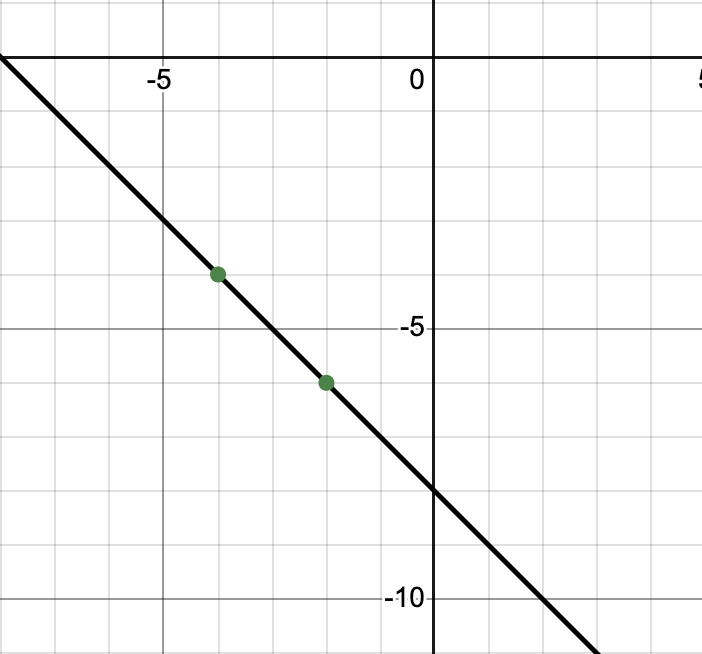
\includegraphics[width=0.3\linewidth]{f10.png}
\end{center}
The graph of the linear function $y = f(x) - 19$ is shown.

If $c$ and $d$ are positive constants, which equation could define $f$?

\textbf{Options:}
\begin{itemize}
    \item[(A)] $f(x) = d - cx$
    \item[(B)] $f(x) = -d + cx$
    \item[(C)] $f(x) = d + cx$
    \item[(D)] $f(x) = -d - cx$
\end{itemize}
\end{frame}

\begin{frame}{\textbf{Answer Explanation: Line with Negative Slope and Vertical Shift}}
\small
We are told that the graph shown is for $y = f(x) - 19$. That means the line shown is the function $f(x)$ shifted down by 19.

To recover $f(x)$, we shift the graph up by 19 units.

From the graph:
\[
\text{The line has negative slope} \Rightarrow f(x) = \text{something with } -cx
\]

We also observe that the $y$-intercept of the graph is approximately $-4$ (which becomes $15$ after adding $19$).

So the general form must be:
\[
f(x) = d - cx, \quad \text{with } d > 0,\ c > 0
\]

Hence, the correct form is:
\[
\boxed{f(x) = d - cx}
\Rightarrow \textbf{Answer: (A)}
\]
\end{frame}


\begin{frame}{\textbf{Question: Percent Decrease as a Factor}}
\small
The expression $kx$ represents the result of decreasing a positive force, $x$, acting on an object by $0.34\%$.

What is the value of $k$?

\textbf{Options:}
\begin{itemize}
    \item[(A)] $0.34\%$
    \item[(B)] $1.34\%$
    \item[(C)] $99.66\%$
    \item[(D)] $100.34\%$
\end{itemize}
\end{frame}


\begin{frame}{\textbf{Answer Explanation: Subtracting Percent from 100\%}}
\small
The expression $kx$ reflects a reduction of $x$ by $0.34\%$.

That means $k$ must represent $100\% - 0.34\% = 99.66\%$ of $x$:
\[
k = 1 - 0.0034 = 0.9966
\Rightarrow \boxed{k = 99.66\%}
\]

\textbf{Answer: (C)}
\end{frame}


\begin{frame}{\textbf{Question: Interior Angle Expression in Terms of } $p$}
\small
A polygon has exactly 87 sides. If the measure of each of the 87 interior angles of this polygon is $(180p)^\circ$, what is the value of $p$?

\textbf{Options:}
\begin{itemize}
    \item[(A)] $\dfrac{85}{87}$
    \item[(B)] $\dfrac{37}{87}$
    \item[(C)] $\dfrac{87}{90}$
    \item[(D)] $\dfrac{87}{180}$
\end{itemize}
\end{frame}


\begin{frame}{\textbf{Answer Explanation: Interior Angles of a Polygon}}
\small
For an $n$-gon, the sum of interior angles is:
\[
(n - 2) \cdot 180^\circ
\]

If each angle is equal:
\[
\text{Each angle} = \frac{(n - 2) \cdot 180}{n}
\]

Given $n = 87$, so:
\[
\text{Each angle} = \frac{(87 - 2) \cdot 180}{87} = \frac{85 \cdot 180}{87}
\]

Also given:
\[
\text{Each angle} = 180p \Rightarrow 180p = \frac{85 \cdot 180}{87}
\Rightarrow p = \frac{85}{87}
\]

\[
\boxed{p = \frac{85}{87}} \quad \textbf{(Answer A)}
\]
\end{frame}


\begin{frame}{\textbf{Question: Exponential Sequence Term Comparison}}
\small
The function $f(n) = 7(20.44)^{\frac{n}{4}}$ gives each term of a sequence as a function of the term's position $n$ in the sequence, where $n$ is a whole number.

The value of the term in position 14 is $p\%$ more than the value of the term in position 10.

What is the value of $p$?
\end{frame}


\begin{frame}{\textbf{Answer Explanation: Percent Increase Between Terms}}
\small
We are given:
\[
f(n) = 7(20.44)^{\frac{n}{4}}
\]

Find:
\[
f(10) = 7(20.44)^{\frac{10}{4}} = 7(20.44)^{2.5} \\
f(14) = 7(20.44)^{\frac{14}{4}} = 7(20.44)^{3.5}
\]

Then compute:
\[
\frac{f(14)}{f(10)} = \frac{7(20.44)^{3.5}}{7(20.44)^{2.5}} = (20.44)^{1} = 20.44
\]

So:
\[
f(14) \text{ is } 20.44 \text{ times } f(10) \Rightarrow \text{increase is } 20.44 - 1 = 19.44
\Rightarrow p = 1944\%
\]

\[
\boxed{p = 1944}
\]
\end{frame}


\begin{frame}{\textbf{Question: Determining the Height of a Pyramid}}
\small
A right square pyramid has a total surface area of $28,\!160$ square inches, and the combined surface area of the four lateral faces of this pyramid is $16,\!060$ square inches.

What is the height, in inches, of this pyramid?

\textbf{Options:}
\begin{itemize}
    \item[(A)] $48$
    \item[(B)] $55$
    \item[(C)] $73$
    \item[(D)] $110$
\end{itemize}
\end{frame}


\begin{frame}{\textbf{Answer Explanation: Solve with Geometry Formulas}}
\small
We are told:
\begin{itemize}
    \item Total surface area: $28,\!160$
    \item Lateral surface area: $16,\!060$
\end{itemize}

The base area is:
\[
\text{Base area} = 28,\!160 - 16,\!060 = 12,\!100

\Rightarrow \text{Base is a square, so: } s^2 = 12,\!100 \Rightarrow s = \sqrt{12,\!100} = 110
\]


\end{frame}

\begin{frame}{Explanation}
Each lateral face is a triangle:
\[
\text{Area of one face} = \frac{1}{2} \cdot 110 \cdot \ell, \text{ where } \ell \text{ is slant height}

\Rightarrow 4 \cdot \frac{1}{2} \cdot 110 \cdot \ell = 16,\!060
\Rightarrow 220 \ell = 16,\!060 \Rightarrow \ell = 73
\]

Now use Pythagoras to find height $h$:
\[
h^2 + \left(\frac{110}{2}\right)^2 = 73^2
\Rightarrow h^2 + 55^2 = 5329

\Rightarrow h^2 + 3025 = 5329

\Rightarrow h^2 = 2304

\Rightarrow h = \sqrt{2304} = \boxed{48}
\]
    
\end{frame}


\begin{frame}{\textbf{Question: One Real Solution Condition for Radical Equation}}
\small
In the given equation, $k$ is a constant. The equation has exactly one real solution.

What is the minimum possible value of $4k$?

\[
\sqrt{k - x} = 32 - x
\]
\end{frame}


\begin{frame}{\textbf{Answer Explanation: Graphical and Algebraic Intersection}}
\small
We are given:
\[
\sqrt{k - x} = 32 - x
\]

**Step 1:** Domain conditions:
\[
k - x \geq 0 \Rightarrow x \leq k \quad \text{and} \quad 32 - x \geq 0 \Rightarrow x \leq 32
\]

So the solution must satisfy $x \leq \min(k, 32)$.

**Step 2:** To have **exactly one solution**, the graphs of both sides must be tangent at that solution.

Square both sides:
\[
k - x = (32 - x)^2 = 1024 - 64x + x^2
\]

Bring all terms to one side:
\[
x^2 - 63x + 1024 - k = 0
\]

For exactly one solution, discriminant must be zero:
\[
\Delta = (-63)^2 - 4(1)(1024 - k) = 3969 - 4096 + 4k = 0
\Rightarrow 4k = 127 \Rightarrow \boxed{4k = 127}
\]
\end{frame}




















\end{document}